\section{Fault-Injection Framework}
\subsection{Whole-Brain Spiking Substrate}
We adopt the released whole-brain LIF model of \emph{Drosophila}\cite{shiu2024drosophila} (Section~\ref{sec:introduction}), implemented in Brian2\cite{goodman2009brian} and built on the FlyWire connectome\cite{lin2024network}. Every neuron is a current-based LIF unit (threshold $-45$\,mV, reset $-52$\,mV, membrane time constant 20\,ms, refractory 2.2\,ms, axonal delay 1.8\,ms). Each connection in the released table becomes a delta-conductance synapse whose jump is $0.275$\,mV per counted contact and decays with a 5\,ms synaptic time constant, signed by the presynaptic cell's neurotransmitter; the table yields 15{,}091{,}983 connections between 138{,}639 neurons (54.5M contacts), 40\% inhibitory. As in the released model, baseline firing is zero: the only external input is the stimulus Poisson group over the driven set, so every recorded spike traces back to the stimulated cells. Our engine restores the full network state at the start of every trial, so all conditions share identical initial states, while the stimulus draws a fresh realization each trial: reported dispersion includes stimulus variability. One 600\,ms trial runs in ${\approx}3.5$\,s on one CPU core.

\subsection{Task: Visuomotor Escape}
The instrumented pathway (Fig.~\ref{fig:system}) is the fly's looming-triggered escape circuit: looming-sensitive visual projection neurons LC4 (104) and LPLC2 (210) converge on descending neurons\cite{shuang2023opplod,simpson2023descending}. Because collision-sensing models treat looming as sustained high-rate drive, we drive the sensory cells---and, as a control, an equal-sized random set---with independent 150\,Hz Poisson trains gated per trial, rather than modeling looming kinetics. The primary readout is the population rate of the command set \{DNp01, DNa02, DNp04, DNb01\} (8 neurons); all 1{,}299 descending neurons serve as a secondary readout. Calibration drove the command population to $94.6$\,Hz (interdecile 93.6--95.8\,Hz, first-spike latency 4.4\,ms; 10-trial set) under escape stimulation but only 8.2\,Hz (6.4--9.2\,Hz) under random stimulation; $\theta=51.4$\,Hz (the 94.6/8.2\,Hz midpoint), every pass/fail classification below is unchanged for thresholds between the observed trial extremes (9.2--63.1\,Hz); Section~IV uses the 12 sweep trials.

\begin{figure}[tb]
\centering
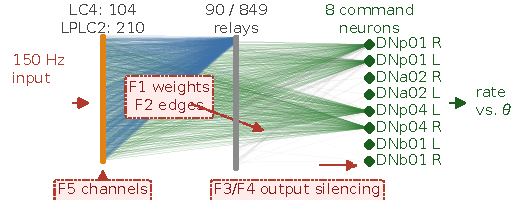
\includegraphics[width=0.96\columnwidth]{figs/fig0_pathway.pdf}
\caption{The instrumented escape pathway, drawn from the connectome itself. Left: the 314 driven sensory cells (LC4, LPLC2); center: the 90 top-ranked of 849 two-hop relays; right: the 8 command DNs. Line width and opacity scale with synapse count (594 direct sensory$\to$DN edges); dashed red marks the fault-injection points (F5 channels; F1/F2 synapses; F3/F4 units). Inset: reconstructed adult brain, adapted from Dorkenwald et al.\cite{dorkenwald2024neuronal} (CC~BY~4.0).}
\label{fig:system}
\end{figure}

\subsection{Fault Taxonomy}
Five fault families cover the hardware-relevant failure modes. F1 multiplies every synaptic weight by an i.i.d.\ mean-preserving lognormal factor ($\sigma\in\{0.05,0.1,0.2,0.5\}$), modeling analog weight variability and bit-level imprecision. F2 deletes a random fraction $f\in\{0.05,0.10,0.25,0.50\}$ of synapses, modeling interconnect or memristor failures. F3 silences all output synapses of a random fraction $f\in\{0.01,0.02,0.05,0.10\}$ of units, excluding input and readout cells (unit removal in this delta-synapse model), modeling dead cores. F4 applies the same operation to the top 1\%, 2\%, or 5\% of units ranked by total outgoing synapse count (again excluding input and readout), modeling failure of high-fanout components; these cells carry 9--22\% of all connections (1\%, 2\% and 5\% sets, respectively), a targeted, correlated version of F3. F5 zeroes all outgoing synapses of one (LC4 or LPLC2) or both sensory channels, modeling sensor or afferent-path failure. All faults are applied after state restoration; F4 and F5 act on fixed cell sets, while F1--F3 redraw their realization each trial from SHA-256 seeds over (phase, condition, trial)---12 independent draws per condition, exactly reproducible from the archived seeds (the stimulus stream is not re-seeded, so re-runs are statistically equivalent rather than bit-identical).\footnote{Code, connectome-derived edge lists, and per-trial records: \url{https://github.com/Scophield/drosophila-fault-injection}.}

\subsection{Controls}
Two controls isolate what the biological wiring contributes. The first is an edge-permuted null: every synapse keeps its presynaptic partner, weight, and sign, but its postsynaptic target is randomly reassigned. This preserves out-degrees, weights, and the global in-degree histogram while destroying which inputs converge onto each target---and with them all multi-hop structure; the identical sweep runs on it. The second is analytic: for both graphs we compute the \emph{pathway mass} $m_k=\mathbf{1}_{\mathrm{DN}}^{\top}A^{k}\mathbf{1}_{\mathrm{in}}$, the synapse-weighted total of all $k$-hop directed paths from LC4$\cup$LPLC2 into the full descending layer ($A$ holds contact counts, i.e., absolute signed strengths; $m_k$ counts $k$-step walks of either sign---a wiring-density proxy, not signal flow), on the intact graph and after the F2 deletion levels; comparing its decay with the output decay separates topological redundancy from dynamical amplification.

